\section{\texorpdfstring{Project description}{Project description }}\label{project-description}

\subsection{From Artificial Generic Intelligence (AGI) to Artificial
Robotic Intelligence (ARI) for the Industry5.0
revolution}\label{from-artificial-generic-intelligence-agi-to-artificial-robotic-intelligence-ari-for-the-industry5.0-revolution}

Artificial General Intelligence (AGI) is an artificial intelligence that
can understand, learn, and apply knowledge across a wide range of tasks
at a human-like level. Unlike narrow AI, designed to perform specific
tasks, AGI would have the ability to think, reason, and solve problems
in a generalized way, like human cognitive abilities. Several key
features characterize AGI: \textbf{Versatility}, \textbf{Learning} and
\textbf{Adaptation}, \textbf{Reasoning} and \textbf{Problem-Solving,
Common Sense and Understanding,} and \textbf{Self-improvement}.
Significant challenges, such as understanding human cognition, creating
adaptable learning algorithms, and developing the computational power
required, must still be overcome despite the high quality reached
recently by tools like ChatGPT4 o1 and Claude 3.5 Sonnet and Gemini.

\textbf{AGI} is commonly considered the edge technology that will
eventually achieve the ambition of \textbf{cognitive robotics,} which
has been the ultimate research goal for the last two decades in
industrial robotics and plays a fundamental role in the success of
Industry5.0. The recent revolution of the \textbf{LLMs} is opening the
question of \textbf{when} robots can integrate such tools and become
\textbf{cognitive agents} in manufacturing.

As a human being, however, the robot is not only \textbf{AI fleshed
out,} but the cognitive abilities rely on conceiving a multiple
interacting system composed of different tools and agents.
\brand{Plan4ARI} aims to step towards a vast scientific leap, following
a \textbf{systematic approach}.

\brand{Plan4ARI} identifies four levels where AI can dramatically
improve the usage of robots in an industrial context.

\begin{itemize}
\item
  A robot is intelligent if the user can describe the task to be tackled
  instead of coding
\item
  A robot is intelligent if it can autonomously solve how to tackle a
  task, considering other agents (robots or humans) inside the operative
  scene
\item
  A robot is intelligent if it can plan its movement considering the
  context and preserving safety under all the operative conditions
\item
  A robot is intelligent if it can move and react appropriately during
  the execution of tasks according to the scene evolution
\end{itemize}

As humans solve the different steps using different capabilities of the
neuronal system, \brand{Plan4ARI} will conceive and deploy a new
generation of intelligent robots integrating the most advanced cognitive
solutions at the state of the art and beyond. \textbf{Artificial Robotic
Intelligence (ARI)} is a complex system where cognitive modules interact
and cooperate to deploy the \textbf{best robotic companion} for human
workers.

\subsection{The Plan4ARI architecture and the COMAU
controller}\label{the-plan4ari-architecture-and-the-comau-controller}

\subsubsection{Context}\label{context}

\textbf{Imagine a mobile manipulator with a high payload that must
perform several welding applications in a fully unstructured environment
like a huge boat.} The working environment is very harmful and unhealthy
for human workers. The references are weak, and many operations must be
defined onsite.

\textbf{Imagine a human operator controlling several different mobile
robots inside this context.} The operator should be able to describe the
task to the robot by using natural language. Then, they should be
enabled to see the virtual execution of the task. They should be able to
notify of errors and eventually ask for plan refinement. Finally, they
should execute the task and be notified if something unexpected happens.
They should be able to move across the robots safely to check ongoing
progress. \textbf{This is not an image of the future} since most
fundamental branches are available at the state of the art and
technology. They must only be refined and turned inside a new generation
of robotics setup enabled with cognitive capabilities. \textbf{Natural
language to task planning is at the edge of the revolution of Generative
AI tools.} Technically, multi-agent generative AI with Reinforcement
Learning (such as ChatGPT o1 or Claude 3.5 AI Sonnet) turns the request
into a sequence of actions, solving the problem when described. These
tools need proper prompt engineering to improve the quality of the
result, and further tools must be able to verify, check, and correct all
the errors that generative techniques introduce. Adopting deliberative
AI tools to lint the output of generative AI techniques is the frontier
of the research to achieve \textbf{safe, efficient, and optimal task
planning}.

\textbf{AI dramatically improves fully autonomous mobile
manipulators\textquotesingle{} motion plan computation and scene
registration}. The AI-powered motion planner can transform symbolic
goals into geometric targets, extrapolating the information from the
images - with minimal support from the human user - and exploiting
advanced localization and registration tools to make the robot aware of
where it is inside the scene. The humans in the scene should be
identified and tracked with compliance with all the safety regulations,
and their intention should be estimated to optimize the motion plan and,
consequently, the task plan.

\textbf{AI-powered robots are expected to achieve a step-change in
performance while continuously modifying the trajectory according to the
scene evolution and the runtime quality tracker.} The controller must
integrate fast full-state observers to boost the control loop and
minimize different functional goals according to the property of the
task. The online modification of the velocity and the compensation of
external dynamic load are still on the edge of technology. Integrating
learning methodologies will allow for keeping a minimum dimensional
dynamic model to control all the elastic and unmodelled dynamics.

\subsubsection{The conceptual
architecture}\label{the-conceptual-architecture}

\begin{center}
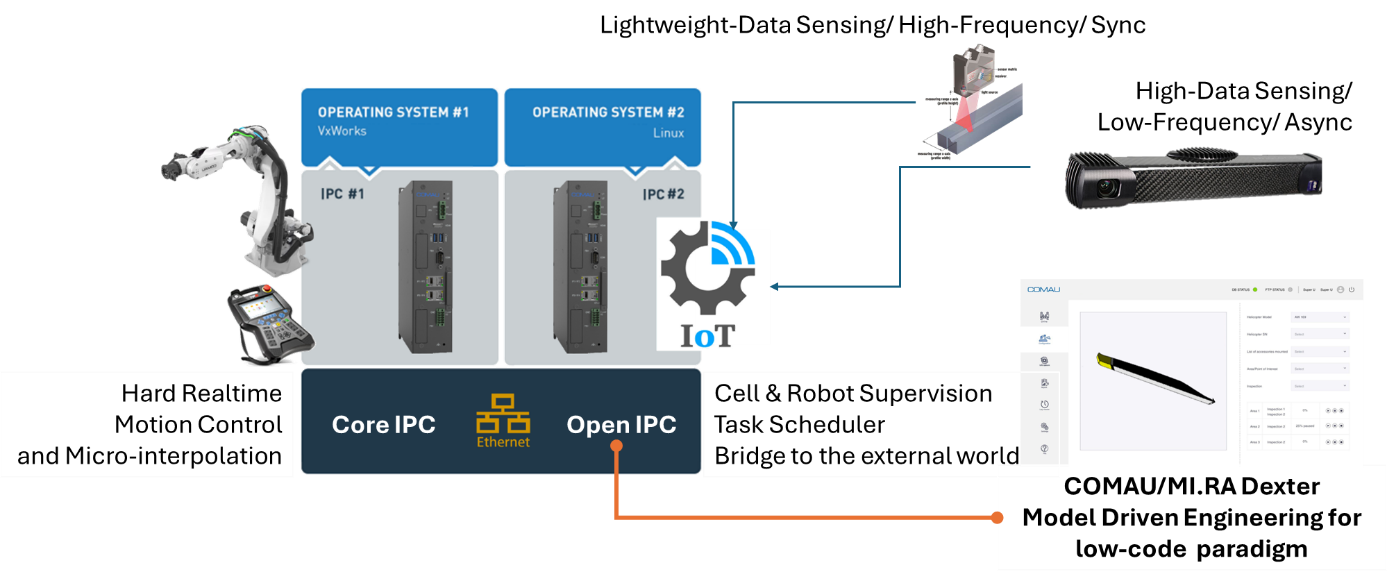
\includegraphics[width=0.96\linewidth,height=0.78\textheight,keepaspectratio]{assets/image1.png}
\end{center}

\planfigurecaption{Figure 1 The Architecture for the new generation of robot controllers needs 2 IPC -- The OPEN IPC provides all the programming tools, the motion planner, and the bridge to the world (cell \& sensing). The Core IPC oversees the control loops and the micro-interpolation (high-rate real-time motion planner) and implements all the safety rules.}

Implementing \textbf{Artificial Robotic Intelligence} requires an
architecture with two control units, as in Figure 1.

First, the \textbf{Open IPC} will be devised with a cognitive
programming platform, the \textbf{MI.RA/Dexter}\footnote{COMAU has
  designed MI.RA/Dexter in the last three years to be a platform capable
  of simplifying the programming of a production line, allowing the
  complete management of a robotic machine from software through the
  creation of a workflow. Dexter can program a line from scratch,
  integrate camera inputs into the system, process images through vision
  algorithms, move the robot via ROS or TCP/IP, manage collision
  avoidance, and more. The idea is to free the production process from
  the need for a specialized worker; the software's end user should be
  able, without having undergone a lengthy learning process, to perform
  the mentioned operations. MI.RA/Dexter aims to achieve a user-friendly
  platform.} from COMAU. This platform is deeply under development in
COMAU and allows two main options for the user: first, it can be fully
customized; second, it consists of a block diagram programming interface
(\textbf{model-driven engineering paradigm}). This block diagram
programming allows the system to store a repository of completed
algorithms, which can be put in a cascade to create a customized process
pipeline. Those available algorithms represent atomic software
functionalities (from simple tasks, such as changing I/O values, to
complex tasks, like collision-free and optimized path planning) that
inherit and extend abstract classes and methods to be compatible with
the underlying software platform. This, in turn, allows the
\textbf{process expert to be the system programmer since it can
completely ignore activities such as user interface, camera calibration,
etcetera}. The Model-Driven, therefore, opens a different cognitive
interaction between human operators and systems, and it will allow in
the future also for the integration of AI modules for the autonomous
generation of process flows (exploiting the co-pilot functionalities
offered by AI that are now in the hype for the code programmers). Using
the classic \textbf{deliberative AI} nomenclature, the
\textbf{MI.RA/Dexter} will be the \textbf{dispatcher} and the
\textbf{execution monitor} engine. The PLC and all the automation will
be connected to the robot controller and \textbf{MI.RA/Dexter} will
deploy full virtualization for the User, controlling and monitoring the
plan execution. \textbf{The Open IPC will bridge the
robot\textquotesingle s control and the external world.} It will
implement the "firewall" between the non-real-time and real-time
automation worlds. It will run powerful tools like ROS2, enabling the
extension of the robot\textquotesingle s capabilities by just connecting
it to external nodes. The \textbf{Open IPC will implement the sensing
and the motion planning interface.} It will provide powerful tools to
plan the motion in every working condition autonomously.

Finally, the \textbf{motion controller} will run on the \textbf{Core
IPC} to grant all the real-time performance and allow the implementation
of advanced control architecture. Furthermore, the \textbf{Core IPC}
will run an advanced hard-real time, high-rate motion planner that will
allow the trajectory modification according to every working condition.
The adoption of innovative strategies will revolutionize the lookahead.

Given such powerful architecture, \brand{Plan4ARI} will, specifically:

\begin{itemize}
\item
  Integrate \textbf{Human-Robot Natural Communication} in the
  \textbf{MI.RA/Dexter platform}. It will consist of a module
  translating the \textbf{natural language} into a \textbf{verified and
  optimal flowchart. A powerful tool to reduce the coding to the minimum
  (e.g., zero for almost all situations)}
\item
  \brand{Plan4ARI} will expand MI.RA/Dexter with further modules for
  \textbf{scene/object registration/segmentation}. The \textbf{operative
  scene} will be \textbf{continuously updated}, and innovative fusion
  techniques to integrate new sensors (like radar) will be implemented
\item
  \brand{Plan4ARI} will expand MI.RA/Dexter with an innovative
  \textbf{motion planner} that will run \textbf{offline} and in
  \textbf{runtime.} The \textbf{points} will be continuously streamed
  from the \textbf{Core IPC} to the \textbf{Open IPC,} which will
  translate the flow of motion references into real-time setpoints for
  the \textbf{hard real-time motion controller}
\item
  \brand{Plan4ARI} will develop an innovative \textbf{Model Predictive
  Controller} for micro-interpolating incoming external references. This
  will revolutionize the lookahead approach in industrial robotics,
  allowing us to achieve impressive tracking performance at Cartesian
  and Joint levels. This innovation will connect the high-rate sensor
  directly to the motion controller to continuously grant the tracking
  performance in every working condition.
\item
  \brand{Plan4ARI} will develop an innovative \textbf{neural
  controller} for \textbf{motion control} with a \textbf{prescribed
  performance constraint} design. This will open a new generation of
  controllers that learn and tune the model, allowing the customization
  of the robotic controller on the system and impressively decreasing
  the deployment time.
\item
  \brand{Plan4ARI} will be natively developed in compliance with the
  \textbf{EU AI Act}, ensuring that all proposed AI solutions adhere to
  the highest standards of safety, transparency, and data protection
  required. The architecture will include specific measures to ensure
  critical AI systems are safe and reliable and respect fundamental
  rights.
\end{itemize}

\subsubsection{Project\textquotesingle s
Modules}\label{projects-modules}

The Project organization is shown in the Figure below. \brand{Plan4ARI}
foresees four modules; each focused on solving a functional aspect of
the cognitive architecture.

\begin{itemize}
\item
  \textbf{Low-code programming and Human-Robot Natural Communication.}
  This module will investigate all the aspects relative to how to
  program the robot using natural language, with the guarantee that the
  autonomously generated program is the best possible. This will be
  discussed in Section \xref{A.3.}
\item
  \textbf{Intelligent Sensing and Safe Motion Planning for Mobile
  Manipulators and Multi-Agents Interaction.} This module will innovate
  both in sensing the scene where the robot is operating and in motion
  planning. The two aspects will hardly be intertwined. The sensing will
  aim to generate a tool that allows a super/accurate registration of
  the robot in the scene and the semantic segmentation of the scene. The
  planner will tackle all the techniques related to path generation,
  considering all the scenarios: offline path generation, online
  re/planning, and high-rate safe hard-real time planning. This will be
  discussed in Section \xref{A.4.}
\item
  \textbf{Advanced Robot Motion Controlling through Machine Learning
  Methods.} This module will investigate a new generation of neural
  controllers to speed up the tuning and increase the tracking
  capability in all possible working conditions. This will be discussed
  in Section \xref{A.5.}
\item
  \textbf{Trustworthiness and Human-Centric Optimization.} This module
  will introduce tools to evaluate users\textquotesingle{} acceptance of
  AI-powered robots. AI could be scary if not correctly managed. The
  module will also investigate how to increase acceptance. This will be
  discussed in Section \xref{A.6.}
\end{itemize}

\begin{center}
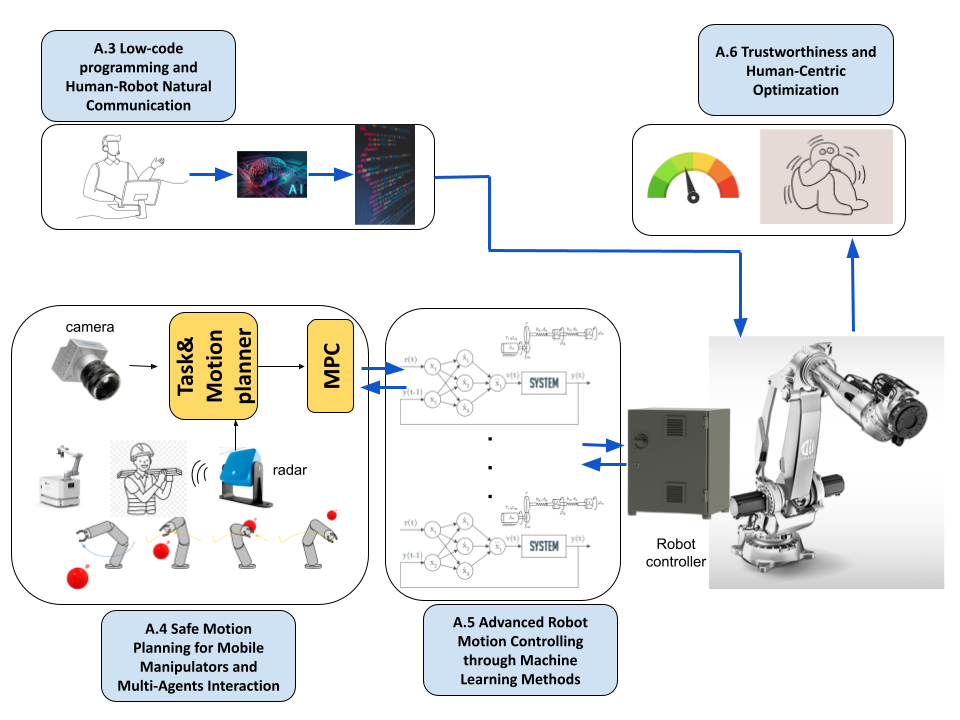
\includegraphics[width=0.72\linewidth,height=0.78\textheight,keepaspectratio]{assets/image2.png}
\end{center}

\planfigurecaption{Figure 2 Graphical Representation of the Plan4ARI modules.}

\subsection{\texorpdfstring{Low-code programming and Human-Robot Natural
Communication
}{Low-code programming and Human-Robot Natural Communication }}\label{low-code-programming-and-human-robot-natural-communication}

\subsubsection{\texorpdfstring{Objectives
}{Objectives }}\label{objectives}

The low-code approach usually asks the user to compose the part program
by dragging and connecting functional modules that perform the sequence
of actions needed to address a task. This approach is the core of the
MI.RA/Dexter low-code programming tool from COMAU. The process expert
usually considers the creation of such a program overwhelming. Model
Driven Engineering is the basis of the low-code approach, and the user
must know all about the libraries the interface has available.
Furthermore, model-driven engineering requires that the user be skilled
in sequential task allocation. Finally, the program composed by the User
is often far from optimal, especially when multi-mobile manipulators are
in the scene or when the human operators cooperate with the robots.

The new generation of cognitive robots should offer the possibility of
\textbf{being programmed using unstructured natural language}. The user
could be unaware of the robot\textquotesingle s functionalities,
automation possibilities, and PLC configurations, and they should be
able to chat with the robot and check the robot\textquotesingle s output
using virtualization of the operations. Edge GenAI, like ChatGPT o1 or
Claude AI 3.5 Sonnet, performs simple reasoning, as shown in the Figure
below.

\begin{center}
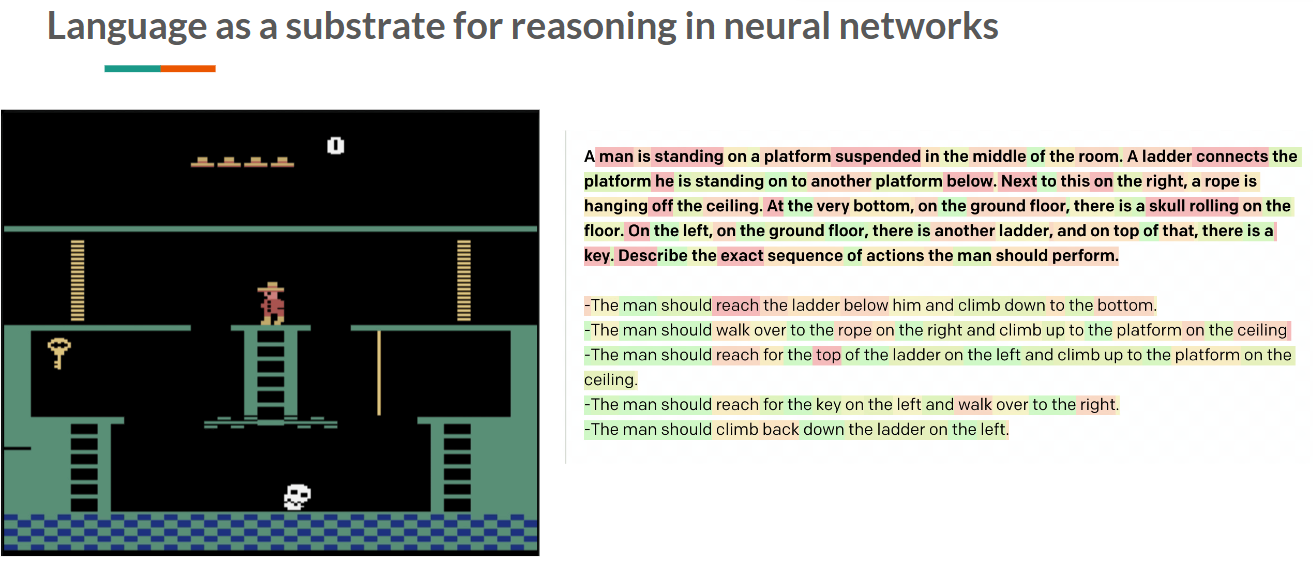
\includegraphics[width=0.76\linewidth,height=0.78\textheight,keepaspectratio]{assets/image3.png}
\end{center}

\planfigurecaption{Figure 3 Example of task planning and prompt engineering (credits to Giambattista Parascandolo, "Language as a substrate for reasoning", seminar at MIT, 2020, link: \url{https://sites.google.com/view/giambattista-parascandolo/home}).}

Significant drawbacks are, however, still blocking the adoption of such
technologies to task planning:

\begin{itemize}
\item
  The prompt must be appropriately engineered
\item
  The output could be erroneous
\item
  The plan is far from being optimum if the problem solution is not
  unique
\item
  The plan cannot consider complex and variable operations
\end{itemize}

\brand{Plan4ARI} aims to be disruptive in translating the natural
language of the human operator into \textbf{Optimal Task Plans} ready to
be executed. \brand{Plan4ARI} will advance the SOTA by putting human
operators at the center of the holistic control framework. Specifically,
we will work to

\begin{itemize}
\item
  \textbf{Innovate methodologies for low-code programming.} The User
  should only be an expert in the process, not an expert in robot
  programming, and not an expert in the functions available in the SW.
  The user interface should enable communication of the desiderata and
  check errors using natural language.
\item
  \textbf{Include the uncertainty of the task duration and the
  interaction,} exploiting data-driven metrics that allow for continuous
  interaction monitoring during the task execution and the
  plan\textquotesingle s evolution to optimize objective cost function
  (like the plan execution).
\item
  \textbf{Optimize task planning, especially for multi-robot systems,
  mobile manipulator teams, and AI-powered robotic companions}. The
  autonomously generated part program, which is ready to be executed,
  will also be optimized. It will consider minimizing the entire
  execution time or other heuristics.
\end{itemize}

\subsubsection{Scientific and Technical
Approach}\label{scientific-and-technical-approach}

\paragraph{Context and
State-of-the-art}\label{context-and-state-of-the-art}

Turning natural language into a task plan is a fundamental research
topic that has been heavily investigated recently. For brevity, a couple
of paradigmatic works on literature are discussed to give context to the
proposed approach.

Focusing on the translation of the natural language in a task plan, an
important recent work\footnote{Singh, I., Blukis, V., Mousavian, A. et
  al. ProgPrompt: program generation for situated robot task planning
  using large language models. Auton Robot 47, 999--1012 (2023).
  \url{https://doi.org/10.1007/s10514-023-10135-3}} explores using LLMs
by creating programming language-style prompts, including function
definitions and environment descriptions. The system enhances PDDL
generation by transforming high-level natural language instructions into
actionable plans. The prompts are designed to fit the
robot\textquotesingle s capabilities and the current environment,
ensuring compatibility between generated actions and the
robot\textquotesingle s capabilities. A further interesting
work\footnote{Lin, K., Agia, C., Migimatsu, T. et al. Text2Motion: from
  natural language instructions to feasible plans. Auton Robot 47,
  1345--1365 (2023). \url{https://doi.org/10.1007/s10514-023-10131-7}} has
extended such an approach to robotics applications. Specifically, the
research aimed at transforming natural language instructions into task
and motion planning (TAMP) for robots using models that combine symbolic
planning with neural networks, like PDDL-based methods. It leverages
deep learning to bridge language and robotic action sequences.

Such approaches, however, are not systematic and have many limitations
in industrial applications, where robustness is fundamental. Indeed,
they do not have deterministic behavior, and it is not possible to have
hard-constrained solutions.

A different approach has been followed in "PDDLStream: Integrating
Symbolic Planners and Blackbox Samplers via Optimistic Adaptive
Planning."\footnote{Garrett, C. R., Lozano-Pérez, T., \& Kaelbling, L.
  P. (2020). PDDLStream: Integrating Symbolic Planners and Blackbox
  Samplers via Optimistic Adaptive Planning.~\emph{Proceedings of the
  International Conference on Automated Planning and
  Scheduling},~\emph{30}(1), 440-448.
  \url{https://doi.org/10.1609/icaps.v30i1.6739}} (2020) -- that focuses on
integrating symbolic planners, like those using PDDL, with LLM-based
black box samplers for task and motion planning (TAMP). The goal is to
generate plans using a combination of high-level language instructions
and learned models for complex robotic tasks. Despite the high quality
of PDDLStream, they weakly support temporal planning, i.e., the scenario
where each task has a predefined duration, and they cannot address
uncertainty in the durations.

A further inspiring work is "Constructing Behavior Trees from Temporal
Plans for Robotic Applications."\footnote{Josh Zapf, Marco Roveri,
  Francisco Martin, Juan Carlos Manzanares, Constructing Behavior Trees
  from Temporal Plans for Robotic Applications,

  \url{https://doi.org/10.48550/arXiv.2406.17379}} mainly focused on a
framework for executing temporal plans in the real and open world, which
requires adapting to environmental uncertainty and planning actions. The
work suggests translating a PDDL plan into a Behavior Tree using a
simple temporal network (STN). The behavior tree (BT) is a convenient
framework for controlling the execution flow of the actions in the plan.
Despite the high quality of such work, the uncertainty of the
task\textquotesingle s duration is not considered.

\paragraph{The Plan4ARI methodology}\label{the-plan4ari-methodology}

Inspired by previous works, \brand{Plan4ARI} will tackle the problem
through a "divide and conquer" approach. Specifically, we will divide
the problem into five steps to ensure that the solution always grants
all the problem constraints and is optimal.

\begin{itemize}
\item
  Step A) State-of-the-art tools of \textbf{Generative AI} will be used
  to deploy a \textbf{Knowledge Base (KB)}. The process engineer will
  check the KB generated architecture, which will be the cornerstone of
  the task planning framework. Multi-agent GenAI with Reinforcement
  Learning (as Claude AI 3.5) will be adopted (\textbf{starting TRL2,
  expected TRL4}). In other words, the creation of KB corresponds to
  pre-form the different functional blocks that can be used, and their
  properties are in a model-driven engineering platform such as
  MI.RA/Dexter.

  \begin{itemize}
  \item
    Task planning is commonly based on the formalization of the
    \textbf{domain}, which consists of defining the \textbf{knowledge
    base.} This can be done according to different toolchains.
    Specifically, an expert in the process will create the KB for a
    class of operations by simply describing the domain using natural
    language. From the description, the tool will extract the domain
    information, such as types (objects or entities), predicates (states
    or conditions), and actions (operations or tasks that change
    states). For example, a proper KB will be created for each class of
    operations, such as welding applications, pick and place, quality
    controls, etc.
  \end{itemize}
\item
  Step B) State-of-the-art tools of \textbf{Generative AI} will be used
  to generate \textbf{PDDL} coherent with the \textbf{KB} from Natural
  Language. The idea consists of exploiting Lightweight LLM. The User,
  therefore, will prompt the description of the specific task, and the
  SW tool will turn it into a PDDL descriptor (\textbf{starting TRL4,
  expected TRL6}).

  \begin{itemize}
  \item
    In literature, the previous step and this step are solved together.
    Generative AI tools generate the PDDL directly from the natural
    description without KB. This, however, can lead to errors in the
    PDDL and weakness in the description. \brand{Plan4ARI} will exploit
    multi-agent generative AI that will check the PDDL according to the
    KB generated at the previous step. A formal verification tool will
    also be exploited. Practically, it does mean that the natural
    language used by the operator to describe the process will be turned
    iteratively in a PDDL until it matches the domain definition stored
    in the KB.
  \end{itemize}
\item
  Step C) Innovative methods will be developed to turn \textbf{PDDL into
  a Behavior Tree with time-variance modeling} to integrate time
  variability. This innovation will allow the \textbf{ARI to tackle
  variable temporal planning without needing} any temporal planner
  solver (\textbf{starting TRL2, expected TRL4}).

  \begin{itemize}
  \item
    At the state of the art, many solvers compute the best task plan
    given the time duration of the tasks. However, no temporal planner
    is still available off-the-shelves that also considers the variance
    in the duration of the tasks, and a few papers are dedicated to this
    issue. Since such a solver is out of the competence of the working
    team, we will follow an alternative path. We will translate the PDDL
    into a behavior tree using time variability to allow a search for
    the best solution over the behavior tree (see next point). This SW
    module will exploit STNU (Simple Temporal Network \textbf{with}
    Uncertainty) and consist of the straightforward extension of
    existing tools that turn PDDL into a Simple Temporal Network
    \textbf{without} Uncertainty (\textbf{starting TRL4, expected
    TRL6}).
  \end{itemize}
\item
  Step D) the \textbf{Task and Motion Planning Optimization} will be
  performed within a \textbf{Digital Twin} Environment.

  \begin{itemize}
  \item
    Having a Behavior Tree that stores all the possible Task plans will
    make it possible to optimize the best task sequence. In the writing
    phase, we aim to explore the multiple parallel BT scenes using
    \textbf{Monte Carlo Tree Search} methodologies, allowing the
    identification of the global optimal plan considering the temporal
    variance of the actions (\textbf{starting TRL2, expected TRL4}). The
    digital twin will consist of turning the BT representation into the
    MI.RA/Dexter flowchart and generate a virtual execution of all the
    tasks.
  \end{itemize}
\item
  Step E) A SW module will execute the Optimal Behavior Tree and will
  implement Online~replanning strategies according to the context state
  (\textbf{starting TRL4, expected TRL6})

  \begin{itemize}
  \item
    The online replanning methodologies will be deployed using
    heuristics. The feasibility during the execution will be the primary
    target since the optimization could ask for a computation time that
    mismatches the execution deadlines and requirements.
  \end{itemize}
\end{itemize}

\subsubsection{\texorpdfstring{Roles and Activities Management
}{Roles and Activities Management }}\label{roles-and-activities-management}

\paragraph{PI Role}\label{pi-role}

The PI will coordinate the activity and be part of the team that designs
the methodology, its deployment, implantation, and testing.

The full team will have a one-week touch point focused on presenting the
results to the PI and the Host Institution Responsible for the
MI.RA/Dexter platform.

\paragraph{Research Organization}\label{research-organization}

The research organization will invest more than 30\% of the budget. The
team will be composed of a Senior Researcher and a fellow.

They will define the methodology and implement it using the first ad-hoc
platform and then (from half-project to the end) inside MI.RA/Dexter.

\paragraph{Host Institution}\label{host-institution}

The Host Institution will invest about 35\% of the budget. The team will
comprise the top figures responsible for the cognitive platform
development, the development team, and the innovation team.

The innovation team will lead the project\textquotesingle s goal, and it
will lead the development of a use case that will verify the quality of
the outcomes.

The development team will continuously interact with the Research
Organization to include the scientific methodologies inside the
platform. At the same time, it will continuously interact with the
research organization team to share typical simulation environments and
tools.

\subsubsection{\texorpdfstring{Expected Results and Key Performance
Indexes
}{Expected Results and Key Performance Indexes }}\label{expected-results-and-key-performance-indexes}

This module will output a unique SW platform able to translate the
natural language into a part program ready to be executed. The
high-level expected results are:

\begin{itemize}
\item
  Programming Time Reduction of 66\%
\item
  Programming performed by not pre-trained worker
\item
  Management of fleet composed of 3 mobile manipulators or 4 industrial
  robotic arms
\end{itemize}

The performance indexes will be measured in controlled environments
designed to test, while the whole system will be evaluated through a
specific demonstrator.

\paragraph{Correctness in the Knowledge Base
Generation}\label{correctness-in-the-knowledge-base-generation}

Different application scenarios will be tested. The autonomously
generated KB will be checked by a human researcher in the field to
verify the accuracy of the results. Furthermore, an automatic KB checker
will be deployed.

\textbf{KPIs:} 10 contexts will be evaluated. \textbf{\textbar{} TRL:}
Such technology is TRL2 in SOTA. Our approach will increase performance;
the novel approach will reach TRL4 (Fundamental Research).

\paragraph{Correctness in the PDDL
generation}\label{correctness-in-the-pddl-generation}

Different application scenarios will be tested, and the output will be
checked by a researcher in the field

\textbf{KPIs: +}100 contexts will be evaluated. \textbf{\textbar{} TRL:}
Such technology is TRL2 in SOTA. Our approach will increase performance;
the novel approach will reach TRL4 (Fundamental Research and Industrial
Research).

\paragraph{Correctness in the BT
generation}\label{correctness-in-the-bt-generation}

Different application scenarios will be tested, and the output will be
checked by a researcher in the field

\textbf{KPIs: +}100 contexts will be evaluated. \textbf{\textbar{} TRL:}
Such technology is TRL4 in SOTA. Our approach will increase performance;
the novel approach will reach TRL6 (Industrial Research).

\paragraph{Optimal Task Planning
Evaluation}\label{optimal-task-planning-evaluation}

Different application scenarios will be tested, and the output will be
checked by a researcher in the field

\textbf{KPIs: +}100 contexts will be evaluated. \textbf{\textbar{} TRL:}
Such technology is TRL2 in SOTA. Our approach will increase the
performance, but the novel approach will reach TRL4 (Industrial
Research).

\subsection{Intelligent Sensing and Safe Motion Planning for Mobile
Manipulators and Multi-Agents
Interaction}\label{intelligent-sensing-and-safe-motion-planning-for-mobile-manipulators-and-multi-agents-interaction}

\subsubsection{\texorpdfstring{Objectives
}{Objectives }}\label{objectives-1}

The definition of the task plan is closely related to the definition of
the movement to perform it. Nowadays, the operative scene is composed of
a variety of agents. Multi-mobile-manipulator teams or humans could be
inside the operative scene, whether with or without fences. Such
challenge scenarios led to a re-think of the definition of robot path
and trajectory, considering the challenging implementation of the
ISO/TS15066 cooperation rules. Such motion planning methodologies are
eventually intertwined with sensing technologies to create awareness of
the operative scene. This is fundamental to implementing scene semantic
segmentation, symbol-to-geometry autonomous capability, and tracking all
humans inside the scene.

In such a context, \brand{Plan4ARI} will deploy a fully autonomous
toolchain for motion planning in \textbf{every working condition}. In
detail, \brand{Plan4ARI} will focus on:

\begin{itemize}
\item
  \textbf{A flexible software tool to solve path planning problems in
  every condition.} The core of this tool will be a library that
  streamlines motion replanning challenges with minimal code
  requirements. It will serve as a valuable resource for researchers
  aiming to develop new algorithms while simplifying the practical
  application of solutions. This tool will implement a \textbf{framework
  to manage the offline planning} and \textbf{online continuous
  replanning.} A software architecture will be devised to oversee the
  execution of the robot\textquotesingle s trajectory, continuous scene
  updates, and concurrent replanning.

  \begin{itemize}
  \item
    \textbf{We will investigate an innovative multi-path replanning
    algorithm.} The algorithm will be designed for fast and efficient
    path replanning, even when dealing with robots with numerous degrees
    of freedom. Instead of aiming to find an entirely new solution to
    reach the goal, the algorithm focuses on connecting to pre-existing
    paths that lead to the same goal. This approach accelerates the
    initial solution discovery process, which can be refined over time.
    Formal guarantees about the completeness and optimality of the
    method are provided, ensuring its reliability.
  \item
    \textbf{We will optimize the motion planning according to the time
    variability of uncontrollable concurrent tasks.} For example, when a
    human operator or moveable objects in the scene cross the robot
    workspace. In such a scenario, a \textbf{safety-aware cost function}
    will be designed to guide the replanning in generating solutions
    prioritizing safety compliance. The resulting algorithm will
    facilitate improved multi-agent cooperation, enabling the robot to
    efficiently adjust its motion in response to the
    operator\textquotesingle s unexpected movements in unstructured
    tasks and environments.
  \item
    \textbf{We will conceive fast replanning strategies} that can
    consider all the dynamics and environmental constraints for runtime
    velocity modulation to improve tracking performance and react to
    sudden scene modifications. Lookahead micro-interpolator fails in
    challenging operative scenes, and innovative approaches that come
    from control science will be investigated and applied. Specifically,
    the motion planning will be designed as modules running over
    different computation units according to the goals (Figure 1). For
    example, on the one hand, the motion planner could run under the
    \textbf{Open IPC} where the user interface is running when the plan
    can be computed asynchronously (offline or online), and the
    computation latency is not critical. On the other hand, the motion
    planning problem must be solved in the \textbf{Core IPC} (Figure 1),
    when the interpolation must be solved in synchronously to the
    process execution (e.g., visual servoing)
  \end{itemize}
\item
  \textbf{Deep learning techniques for autonomous robot registration}
  inside the scene and \textbf{semantic segmentation} of the
  scene\textbf{.} The autonomous generation of the motion plan needs the
  exact localization of the robot into the scene. This will be performed
  autonomously by adopting a mix of hand-to-eye and eye-to-hand sensing
  systems. Furthermore, a robust segmentation engine will translate the
  symbolic description of Cartesian targets into the exact localization
  of such poses.
\item
  \textbf{The integration of radar sensors to track the human inside the
  scene.} The objective will be to test and deploy algorithms that can
  exploit both 3D point clouds coming from vision systems and radar
  sensors. Radar sensors are the most promising technology for boosting
  human-robot interaction.
\end{itemize}

\subsubsection{Scientific and Technical
Approach}\label{scientific-and-technical-approach-1}

\paragraph{Context and
State-of-the-art}\label{context-and-state-of-the-art-1}

Generating a new path whenever a new obstacle appears requires
substantial computational resources and time. A more efficient approach
involves dynamic adjustment of the existing path to quickly and
efficiently respond to changes. Nevertheless, existing techniques still
require significant computational power, impacting their responsiveness.
Replanning algorithms need to be supported by complex software
architectures. When dealing with unchanging environments, the regular
approach to motion planning involves computing a path, assigning it a
time parametrization, and executing the resulting trajectory. On the
other hand, when it comes to motion replanning, there is a greater
demand throughout the trajectory\textquotesingle s execution. It is
essential to consistently reevaluate and adjust the plan as the robot
moves, smoothly transitioning to new trajectories. \textbf{This calls
for an architecture that not only supervises the robot\textquotesingle s
motion execution but also maintains up-to-date scene information while
simultaneously managing the replanning process.} However, in workspaces
shared with humans, it is necessary to do more than ensure that the
robot\textquotesingle s path is collision-free. The
robot\textquotesingle s speed adjustments and halts are controlled by
safety systems that continually monitor the workspace to guarantee human
safety. The ISO/TS 15066 safety standard proposes collaborative
operations like Speed and Separation Monitoring (SSM) or Power and Force
Limiting (PFL) to adhere to safety regulations and protocols. The choice
of strategy depends on risk analysis and aims to reduce potential
hazards.

Their implementation typically limits robot speed and halts when the
human and the robot are close. It is possible to reduce the idle times
caused by the safety intervention by planning robot movements that
minimize the safety speed limitations. Researchers have investigated
this problem at various levels, proposing adaptive task
planners\footnote{S. Sandrini, M. Faroni, and N. Pedrocchi, ``Learning
  action duration and synergy in task planning for human-robot
  collaboration,'' in 2022 IEEE 27th Int Conf on Emerging Technologies
  and Factory Automation (ETFA), 2022, pp. 1--6.}, motion
planners\footnote{A. Palleschi, M. Hamad, S. Abdolshah, M. Garabini, S.
  Haddadin, and L. Pallottino, ``Fast and safe trajectory planning:
  Solving the cobot performance/safety trade-off in human-robot shared
  environments,'' IEEE Robot. Autom. Lett., vol. 6, pp. 5445--5452,
  2021.}, and controllers\footnote{C.-M. Huang and B. Mutlu,
  ``Anticipatory robot control for efficient human-robot
  collaboration,'' in 2016 11th ACM/IEEE Int Conf on Human-Robot
  Interaction (HRI), 2016, pp. 83--90}. Motion planning is pivotal in
this endeavor, with researchers striving to consider the
operator\textquotesingle s presence and trigger the safety module as
sparingly as possible, employing proactive or reactive approaches.
\textbf{Proactive planners} pre-compute trajectories that minimize the
expected interference between the operator and the robot. This relies on
a model of human behavior and the minimization of collision risk,
execution time, or human discomfort. While these approaches are robust
to the operator\textquotesingle s presence, duration and frequency of
access, they become considerably less reliable when the
operator\textquotesingle s position is out of distribution.
\textbf{Reactive planners} focus on real-time robot trajectory
modifications, involving dynamic speed adjustments according to the
distance from the operator and the ability to alter the path
dynamically. Speed reduction works when the intrusions are short and
sparse, but it is inefficient with frequent collaboration, resulting in
safety stops whenever the human is nearby. An emerging trend is to
combine strategies, employing path modifications during execution and
trajectory scaling.

A promising strategy for motion planning in collaborative operations is
blending reactivity with proactivity. This is achieved by integrating a
reactive motion replanning algorithm with a human-aware cost function to
minimize interference proactively. In this way, cooperation efficiency
is improved by optimizing the trajectory for travel times and
operator-induced safety slowdowns. Previous studies were limited to
offline planning when considering human influence\footnote{R. Laha, W.
  Wu, R. Sun, N. Mansfeld, L. F. Figueredo, and S. Haddadin, ``S*: On
  safe and time efficient robot motion planning,'' in 2023 IEEE Int.
  Conf. Rob. Aut. (ICRA), 2023, pp. 12 758--12 764}, and replanning
algorithms could require adaptations to handle more complex cost
functions

In such a context, \textbf{sample-based algorithms, such as rapidly
exploring random trees (RRT)} and \textbf{probabilistic roadmaps} (PRM),
are famous for robot trajectory planning because they can efficiently
handle high-dimensional spaces. One of the critical developments in
improving the efficiency of these algorithms is the concept of the
\textbf{informed set}, which is particularly useful for enhancing the
performance of algorithms like RRT*, an optimized version of the
original RRT.

Specifically, the \textbf{informed set} is a subset of the state space
that contains all the potentially be easily integrated into the
replanning solutions to a given problem. In traditional sampling-based
planners, samples are drawn uniformly from the entire state space, which
can lead to inefficiencies, mainly when the feasible region for the
optimal path is small. The informed set constrains the sampling space to
focus on regions more likely to contain the optimal solution,
significantly reducing the number of samples needed. For example, in
RRT*, the informed set is defined as an ellipsoid that bounds the
solution space. The planner converges more quickly to an optimal
solution by focusing sampling within this ellipsoid. This ellipsoid is
defined based on the best path cost and the distance from the start to
the goal state.

The primary advantages of using an informed set in sample-based planning
algorithms include \textbf{Reduced Computational Complexity}: Sampling
within a constrained region (informed set) decreases the number of
required samples, accelerating the convergence toward the optimal
solution, \textbf{Improved Path Quality}: By focusing sampling in
regions that are more likely to contain the optimal solution, informed
set-based methods produce better-quality paths, with fewer iterations,
\textbf{Scalability}: The use of an informed set makes these algorithms
scalable to higher-dimensional spaces, which is crucial for
applications, such as autonomous drones and manipulators operating in
complex environments.

The availability of fast planning methodologies based on sample-based
approaches is decisive for the path design, but it is hard to integrate
the dynamics constraints of the robot. Dynamics computation would insert
an excessive workload in the state exploration and exploitation.

A different approach uses \textbf{Model Predictive Control} (MPC) as an
active filter to generate a robot controller\textquotesingle s path or
trajectory reference. MPC is used for trajectory generation rather than
feedback control in this configuration. \textbf{MPC} can be designed to
calculate a \textbf{sequence of future reference points} for the robot
to follow based on the desired objectives (such as reaching a target
location while avoiding obstacles). MPC solves an optimization problem
over a prediction horizon, considering system dynamics, constraints
(like robot speed, acceleration, and workspace boundaries), and external
factors (such as obstacle positions or dynamic environments). In this
context, the MPC output is a smooth, feasible trajectory that serves as
the \textbf{reference input} for the lower-level controller.

The MPC\textquotesingle s output is smoother and respects the
robot\textquotesingle s physical constraints, ensuring the path is
feasible. This trajectory can be updated in real-time based on feedback,
making it more adaptive to environmental changes or disturbances. There
are multiple key benefits of using MPC for trajectory generation.
\textbf{Constraint Handling}: MPC allows you to account for physical
constraints like maximum velocity, acceleration, and obstacle avoidance
directly in the trajectory generation process. \textbf{Adaptivity}: The
real-time nature of MPC allows for trajectory adjustments in dynamic
environments or under disturbances. \textbf{Smooth and Feasible
Trajectories}: MPC naturally generates smooth, feasible trajectories
that meet the system\textquotesingle s limitations. Model Predictive
Control (MPC) has significantly contributed to the trajectory generation
for autonomous robots, with applications ranging from ground vehicles to
aerial drones.

One relevant study focuses on MPC-based trajectory generation for aerial
robots\footnote{T. Power and D. Berenson, "Learning a Generalizable
  Trajectory Sampling Distribution for Model Predictive Control,"
  in~\emph{IEEE Transactions on Robotics}, vol. 40, pp. 2111-2127, 2024,
  doi: 10.1109/TRO.2024.3370026.}, where the MPC algorithm dynamically
adjusts paths while considering environmental uncertainties. This
approach uses learned penalization functions within the MPC framework to
avoid redundant coverage of already explored areas, optimize the
trajectory for search and coverage missions, and make it ideal for
aerial robotic systems. Another recent paper presents
\textbf{SOMTP}\footnote{Liu, Yifan, You Wang, and Guang Li. "SOMTP:
  Self-Supervised Learning-Based Optimizer for MPC-Based Safe Trajectory
  Planning Problems in Robotics." arXiv preprint arXiv:2405.09212
  (2024).}, a learning-based optimization framework integrated with MPC
for safe trajectory planning in robotics. It uses Control Barrier
Functions (CBFs) to ensure safety around obstacles. The combination of
MPC and CBF allows robots to plan dynamically while respecting real-time
constraints, particularly in highly nonlinear, non-convex environments.
Furthermore, many MPC-based frameworks have been applied for autonomous
vehicle path tracking, enhancing real-time decision-making and path
adjustments under dynamic conditions like obstacle avoidance and lane
changes\footnote{Johny, D., Jisha, V.R. (2023). Model Predictive
  Control-Based Trajectory Generation and~Tracking of~an~Electric
  Vehicle. In: Siano, P., Williamson, S., Beevi, S. (eds) Intelligent
  Solutions for Smart Grids and Smart Cities. IPECS 2022. Lecture Notes
  in Electrical Engineering, vol 1022. Springer, Singapore.
  \url{https://doi.org/10.1007/978-981-99-0915-5_22}}.

A further research challenge consists of tracking and segmenting all the
information in the scene. This point is crucial to:

\begin{itemize}
\item
  Allow \textbf{fully symbolic programming.} In other words, the user
  indicates only a symbolic target to the robot, while the robot
  autonomously converts in Cartesian/Joint targets.
\item
  Tracking the moveable objects in the scene is the boost to enable
  online replanning and -- therefore -- an improvement of the efficiency
  of the systems.
\end{itemize}

Sensing systems based on 3D cameras have achieved high performance in
many conditions. The segmentation of the images is impressively
improving every year, and FOSS algorithms are available. The main issue
related to 3D camera systems is related to the fact that they are slow
to track fast movement (like human movements), and only one camera in
the market is certifiable safe -- to the best knowledge of the PI.

In automotive, it has been more than a decade since the fusion of radar
sensor and camera systems allowed impressive performance and an
intrinsic level of safety. On the one hand, radars are extremely fast,
allowing the updating of the scene status. On the other hand, the
data\textquotesingle s resolution and noise are significantly worse than
the 3D images.

The fusion of camera and radar sensors is highly appealing to robotics.
The most relevant trend considers \textbf{Deep Learning Dominance},
i.e., moving towards deep learning-based fusion, where networks can
learn complex relationships between the sensors. New architectures like
transformers are being explored for better sensor integration. These
methods are also investigated to achieve high performance in
\textbf{sensor calibration and alignment}, ensuring precise spatial
alignment between radar and cameras, and are also advancing. Remarkably,
radar and camera data fusion is evolving rapidly with AI and machine
learning advancements, leading to more accurate, reliable, and safe
autonomous systems.

\paragraph{The Plan4ARI methodology}\label{the-plan4ari-methodology-1}

Being inspired by my previous works in the field and exploiting my FOSS
software (\url{https://github.com/JRL-CARI-CNR-UNIBS/OpenMORE} ),
\brand{Plan4ARI} will tackle the problem through an innovative
framework designed explicitly for motion planning and re-planning.
Precisely, the technical and scientific approach will follow

\begin{itemize}
\item
  Development of an SW module for the \textbf{sensing fusion}. The
  fusion of images and radar sensing systems will be addressed to have a
  high-frequency 3D point cloud of the cell.

  \begin{itemize}
  \item
    The goal is to boost the update frequency of the scene by a double
    sensing layer. The internal fast layer will comprise radar sensing
    technologies that create low-resolution and noisy point clouds at
    high frequencies. The outer layer will be composed of 3D camera
    systems that update the scene state at low frequency, over which it
    is possible to perform accurate registration and segmentation. This
    framework will allow the high-frequency tracking of moveable objects
    in the scene.
  \item
    The module will integrate state-of-the-art fusion and segmentation
    techniques to extract information from 3D colored point clouds. This
    will allow the robot to interface with the object database and
    program the robot using symbols (e.g., descriptors of the objects in
    the scene) and not Cartesian goals. If the system fails in object
    identification, the Cartesian goals will be inserted with an
    easy-to-tune user Cartesian reference frame.
  \end{itemize}
\item
  Development of a tool for advanced understanding of the scene.

  \begin{itemize}
  \item
    First, thanks to the sensing system\textquotesingle s high-rate
    enriched sensing fusion, it will be possible to implement advanced
    state-of-the-art registration methodologies. \textbf{This will allow
    continuously updating the robot\textquotesingle s position in the
    scene.} Like in mobile manipulators, the high localization will
    allow to tackle straightforwardly the semantic segmentation
  \item
    Module A3 will allow the creation of the KB of each scenario easily.
    This powerful tool will enable the implementation of advanced
    semantic segmentation techniques. The segmentation and pose
    estimation of the objects of the scene will allow for the symbolic
    planning of the robot. No Cartesian poses will be necessary anymore
    when programming the Robot.
  \end{itemize}
\item
  Development of adaptive strategies across task planning and motion
  planning to minimize the need for safety interventions -- that means
  to reduce wasted time and enhance collaborative productivity.
  \textbf{Building upon the existing safety module,} we will deploy
  sample-based strategies that \textbf{proactively} and
  \textbf{reactively} oversee the robot\textquotesingle s actions,
  ensuring smooth cooperation with the operator in shared spaces. I aim
  to bridge the gap between safety-aware proactive and reactive methods.

  \begin{itemize}
  \item
    The conventional approach to path replanning needs will be
    reconsidered. Ensuring a collision-free trajectory does not
    necessarily translate to a safety-compliant robot\textquotesingle s
    behavior. Modifying the path to avoid collisions might cause the
    safety system to intervene significantly, resulting in slowdowns or
    stops, which could undermine the robot\textquotesingle s
    effectiveness. As a result, replanning algorithms need to be aware
    of the effects of the safety module. These algorithms will consider
    humans as obstacles and factors that affect how the trajectory
    should be modified to achieve efficient behavior
  \item
    The approach I will pursue will integrate a safety-aware cost
    function based on ISO/TS 15066 into a fast-replanning algorithm,
    changing the robot\textquotesingle s path in runtime. The primary
    objective is to minimize the execution time of the trajectory,
    considering the estimated speed limitations. The method will address
    the limitations of proactive approaches by allowing online
    adaptation of the plan to accommodate unexpected movements of the
    operator. It also improves the efficiency of reactive approaches,
    going beyond simple collision-free path replanning and actively
    seeking safety-aware solutions, aim to prevent hazardous situations
    instead of reacting to it. For this purpose, we draw inspiration
    from my work\footnote{M. Faroni, M. Beschi, and N. Pedrocchi,
      ``Safety-aware time-optimal motion planning with uncertain human
      state estimation,'' IEEE Robot. Autom. Lett., vol. 7, no. 4, pp.
      12 219--12 226, 2022.} to introduce a safety-aware cost function
    based on ISO/TS 15066 that can be easily integrated into the
    replanning algorithm.
  \item
    To overcome the computational complexity, which can impact robot
    promptness, I will adopt a \textbf{sampling-based approach}. This
    method seeks solutions by randomly sampling the robot search space,
    and it is favored for its simplicity, adaptability, and ability to
    scale, even when dealing with large search spaces (e.g., robots with
    many degrees of freedom).
  \item
    The idea consists of dramatically improving the performance of
    RRT-like sampling-based path planners by combining
    \textbf{admissible informed sampling and local sampling} (i.e.,
    sampling the neighborhood of the current solution). \textbf{An
    adaptive strategy} will regulate the trade-off between exploration
    (admissible informed sampling) and exploitation (local sampling)
    based on online rewards from previous samples.
  \end{itemize}
\item
  Development of a \textbf{Model Predictive Controller} for path
  planning running alongside the adaptive sampling-based motion planner.
  This will integrate the controlled model of the robot to generate the
  best trajectory concurrently with the robot execution task, granting
  the prescribed performance.

  \begin{itemize}
  \item
    The MPC is renowned for its performance in optimizing the control
    law and non-linear complex systems. \brand{Plan4ARI} will focus on
    online speed adaptation to reduce the tracking error when the
    dynamics load is essential for the actuators. Alternatively, the
    robot will exploit the residual degrees of freedom along a path to
    reduce the jerk of the trajectory. For example, suppose the robot
    end-effector can rotate freely along the tool axis (e.g., in many
    welding applications, in machining, and in painting, it happens
    frequently). In that case, the MPC will compute the best orientation
    to reduce the maximum/mean torque for the motors along the required
    time window.
  \end{itemize}
\end{itemize}

\subsubsection{\texorpdfstring{Roles and Activities Management
}{Roles and Activities Management }}\label{roles-and-activities-management-1}

\paragraph{PI Role}\label{pi-role-1}

The PI will coordinate the activity and be part of the team that designs
the methodology, its deployment, implantation, and testing.

The team will have a one-week touch point focused on presenting the
results to the PI, the Host Institution Responsible for the MI.RA/Dexter
platform and the Host Institution are Responsible for the low-level
control.

\paragraph{Research Organization}\label{research-organization-1}

The research organization will invest about 35\% of the budget in this
topic. The team will comprise two fellow researchers directly, followed
by the PI.

They will define and implement the methodology using the ad-hoc platform
and then (from half-project to the end) inside MI.RA/Dexter (for the
offline/online motion planner) and the \textbf{Core IPC} (for the Model
predictive controller).

\paragraph{Host Institution}\label{host-institution-1}

The Host Institution will invest about 35\% of the budget to integrate.
Different top figures will be engaged: the responsible for the cognitive
platform development, the responsible for the low-level controller
development, and the responsible department of the vision systems.

Three working teams will be engaged. First, a working team will mainly
focus on developing innovative methodologies for scene update,
registration, and semantic segmentation. The second working team will
integrate the offline/online motion planner with the MI.RA/Dexter
platform. The second working team will put effort into deploying the
Core IPC controller with a double goal. First, the MPC must be
integrated into the Core IPC. Second, to create a powerful async
communication channel with the MI.RA/Dexter platform for safe continuous
streaming of reference trajectories for the robot.

Both teams will continuously interact with the Research Organization to
include the scientific methodologies inside the platform. At the same
time, it will continuously interact with the research organization team
to share common simulation environments and tools.

\subsubsection{\texorpdfstring{Expected Results and Key Performance
Indexes
}{Expected Results and Key Performance Indexes }}\label{expected-results-and-key-performance-indexes-1}

This module will output a unique SW platform able to translate the
natural language into part program ready to be executed. The high-level
expected results are:

\begin{itemize}
\item
  Fully autonomous generation of the motion plan in all the required
  working conditions. Both joint and Cartesian planning will be
  supported.
\item
  Reduction of the execution time for interaction tasks by 30\% to
  state-of-the-art motion planners.
\item
  Safe adaptation of the velocity according to any working conditions
\end{itemize}

The performance indexes will be measured in controlled environments
designed to test, while the whole system will be evaluated through a
specific demonstrator.

\paragraph{Computation Time Target}\label{computation-time-target}

\brand{Plan4ARI} will test at least 50 application scenarios, and the
output will be checked by benchmarking it with OMPL planners
(\url{https://ompl.kavrakilab.org/index.html}). As a note, the planners
running on GPU will not be compared.

\textbf{KPIs:} Computation time, computed as mean over \textbf{+}100
contexts. \textbf{\textbar{} TRL:} Such technology is TRL5 in SOTA. Our
approach will increase performance, but the novel approach will reach
TRL7 (Industrial Research).

\paragraph{Scene Update Target}\label{scene-update-target}

\brand{Plan4ARI} will test at least 50 Different application scenarios.
The sensor fusion of radar technologies and 3D images will be tested
over the standard 3D vision-based systems.

\textbf{KPIs:} The accuracy in the registration in +100 contexts will be
evaluated. The fused information is expected to grant a better accuracy
of about 20\% using standard registration policy (e.g., IPC)
\textbf{\textbar{} TRL:} Such technology is TRL4 in SOTA. Our approach
will increase performance, and the novel approach will reach TRL6
(Fundamental Research).

\paragraph{\texorpdfstring{Trajectory adaptation to reduce dynamics load
}{Trajectory adaptation to reduce dynamics load }}\label{trajectory-adaptation-to-reduce-dynamics-load}

\brand{Plan4ARI} will test at least 50 Different application scenarios.

\textbf{KPIs:} The tracking performance will be increased by about 50\%
\textbf{\textbar{} TRL:} Such technology is TRL5 in SOTA. Our approach
will increase performance, and the novel approach will reach TRL7
(Industrial Research).

\subsection{\texorpdfstring{Advanced Robot Motion Controlling through
Machine Learning Methods
}{Advanced Robot Motion Controlling through Machine Learning Methods }}\label{advanced-robot-motion-controlling-through-machine-learning-methods}

\subsubsection{\texorpdfstring{Objectives
}{Objectives }}\label{objectives-2}

The inner layer of the \brand{ARI} (Figure 1) is the high-rate
real-time motion controller. In such a context, the system
identification and control law design are interweaved, and edge
generative AI technologies are scarce in challenging domains like
robotics, where \textbf{high non-linearity poses significant
challenges}. Recent pioneering approaches tackle the new generation of
AI-driven motion controllers by learning meta-dynamical models of a
high-dimensional physical system to be integrated with Deep Model
Predictive Control frameworks in robotics. Others integrate lightweight
networks inside the motion control law.

Significant drawbacks are, however, still blocking the adoption of
advanced learning-based control strategies in industrial robot
controllers:

\begin{itemize}
\item
  The computational burden
\item
  The robustness and adaptability
\item
  The integration with the robot sensing (e.g., vision and force
  sensors) and their performance
\end{itemize}

\brand{Plan4ARI} aims to be disruptive in conceiving and deploying a
new generation of motion controllers that put the adaptivity to variable
scene conditions at the center - i.e., that preserves safety and
controllability in every condition.

\begin{itemize}
\item
  \textbf{To innovate in deploying controllers that guarantee
  performance even under actuator faults and motion constraints.} The
  goal consists of innovating the tracking control problem of robotic
  systems with guaranteed transient behavior and steady-state
  performance in the presence of modeling uncertainties, unexpected
  actuation failures, and motion constraints.
\item
  \textbf{To innovate in deploying controllers considering elasticity
  inside the industrial robot joints.} The goal is to innovate robotic
  systems\textquotesingle{} tracking control problem when the
  joints\textquotesingle{} elastic effect is not neglectable.
\item
  \textbf{To innovate in the robustness and reliability of neural
  controllers.} Given the hard real-time and control robustness
  requirements, AI applied to robot control is challenging. Plan4ARI
  will boost a new generation of adaptive neural controllers designed
  with \textbf{learning policies that can run over lightweight
  industrial PCs} - i.e., the most powerful CPUs will never control
  industrial robots.
\end{itemize}

\subsubsection{Scientific and Technical
Approach}\label{scientific-and-technical-approach-2}

\paragraph{Context and
State-of-the-art}\label{context-and-state-of-the-art-2}

A common trend in industrial robotics is to couple full-state observers
with fine-tuned axis controllers, where the identification of the robot
dynamics plays a fundamental role.

This classical approach relies on important assumptions: it allows a
complete physical understanding of the control law, debugging, and the
fact that the robot model can be fully deployed. However, the elastic
modeling of the robot introduces severe limitations, given the high
order and the relative modeling complexity.

The literature reports an incredible number of possible full-state
observers to estimate the complete state of a system (e.g., positions,
velocities, accelerations) when some parts of the state are not directly
measurable. Among the others, the \textbf{Unscented Kalman
Filter}\footnote{\textsuperscript{Siciliano, B., Sciavicco, L., Villani,
  L., \& Oriolo, G. (2010). Robotics: Modelling, Planning and Control.
  Springer Science \& Business Media.}} (UKF) avoids linearization by
using an unscented transform to propagate mean and covariance through
the system\textquotesingle s nonlinear dynamics. This provides better
estimates than the Extended Kalman Filter (EKF) for highly nonlinear
systems. It is used in applications with more pronounced nonlinearities,
such as in high-speed robotic navigation, UAVs, or in cases with
significant sensor noise and complex dynamics. However, it is
computationally expensive and poorly manageable for real-time
applications that run on IPCs. Another observer that is very commonly
used is the \textbf{sliding mode observer}. This is a robust observer
used primarily for systems with uncertainties or disturbances. The
sliding mode observer uses a discontinuous control signal to "slide" the
estimated state to the true state in the presence of disturbances. It is
particularly useful in systems with bounded noise and disturbances.
Sliding mode observers are applied in robotic manipulators and mobile
robots, especially for estimating states in the presence of model
uncertainties or external disturbances. Although it is highly robust to
disturbances and model inaccuracies, it can introduce chattering due to
discontinuous control, though techniques exist to mitigate this. Often,
it is used for force estimation in robotic manipulators or fault
detection in industrial robots.

A recent trend is the adoption of a \textbf{High-Gain Observer} that
grants fast and accurate state estimation (e.g., joint velocities or
forces). However, they are extremely sensitive to noise, and model
inaccuracies can be problematic when using high feedback gains.

An alternative approach to having a high-performing observer is to have
a full neural controller. Neural controllers\footnote{aa} represent a
frontier for industrial robot control because they offer many potential
advantages over traditional control strategies. These advantages are
rooted in the capabilities of neural networks to handle complex,
nonlinear, and dynamic systems, which are common in industrial robotics.
The most interesting properties for neural controller are:

\begin{itemize}
\item
  \textbf{Learning and Adaptability}. Traditional controllers, such as
  PID (Proportional-Integral-Derivative) or model-based controllers, are
  often tuned for specific tasks and environments. They struggle when
  operating in dynamic, uncertain, or unstructured environments that are
  becoming more common in modern industries. The Neural Controllers show
  the advantage that can learn from data, adapting their behavior as
  tasks, conditions, or environments change. This ability to learn and
  generalize from experience allows robots to handle a wider variety of
  tasks without needing to reprogram or fine-tune control parameters.
\item
  \textbf{Handling Nonlinearities and Complex Dynamics.} Industrial
  robots often deal with highly nonlinear systems, such as joint
  friction, backlash, and dynamic loads, which can be difficult to model
  and control using conventional methods. The Neural Controllers show
  the advantage that neural networks excel at approximating complex,
  nonlinear relationships without the need for detailed system models.
  This enables better control of robots with complex dynamics.
\item
  \textbf{Real-Time Adaptation to Unknown Disturbances.} Industrial
  environments are often unpredictable, with variable external forces,
  or sudden changes in load. Conventional controllers require precise
  models and struggle with real-time adaptation to such disturbances.
  The Neural Controllers, particularly those integrated with
  reinforcement learning (RL) or adaptive control methods, can adjust in
  real time to unforeseen disturbances, improving the robot's ability to
  maintain stability and performance even in uncertain conditions.
\item
  \textbf{Data-Driven Control.} In traditional control systems, deriving
  accurate models of robot dynamics or task environments requires
  time-consuming analytical work. Data-driven control simplifies this by
  learning directly from operational data, making the process faster and
  more adaptable to changes. The Neural Controllers show the advantage
  that they use data to ``learn'' system behavior without the need for
  explicit modeling, offering an efficient way to create control
  policies. This is particularly useful when the robot\textquotesingle s
  environment is too complex or unknown for model-based control.
\item
  \textbf{Improvements in Sensing and Perception.} Robots are
  increasingly equipped with advanced sensors, including vision systems,
  force-torque sensors, and haptic feedback devices. Traditional
  controllers often have difficulty integrating and making real-time
  decisions based on this flood of sensory data. The Neural Controllers
  are highly effective at processing large amounts of sensor data, such
  as camera inputs, LiDAR, or touch sensors. This ability enables robots
  to adjust their behavior based on rich sensory input.
\item
  \textbf{Task Generalization and Autonomous Learning.} In many
  industrial settings, robots are required to perform multiple tasks or
  variations of the same task. Conventional controllers usually need to
  be fine-tuned for each task, which limits their flexibility. The
  Neural Controllers, particularly those trained through reinforcement
  learning, can generalize across tasks. They can learn from a broad set
  of experiences and apply those learnings to new, unseen tasks without
  the need for manual reprogramming.
\item
  \textbf{Cost Efficiency and Flexibility}. Traditional robot control
  systems often require expensive hardware and fine-tuned software for
  specific applications, which can be costly and time-consuming to
  develop and maintain. Neural controllers can reduce development time
  and costs by learning directly from data and reducing the need for
  complex, hand-crafted control logic. As neural networks evolve, they
  could also allow for more general-purpose robots to handle a broader
  range of tasks with fewer customizations.
\end{itemize}

Recently, some kinds of neural network (NN) control methods, such as
NN-based inverse control, indirect adaptive NN control, and direct
adaptive NN control, have been proposed to deal with dynamic
uncertainties. Several elegant adaptive neural controls (ANCs) have been
presented for nonlinear systems to simplify controller design and avoid
model estimation. However, the given predefined performance requirements
for the convergence rate, maximum overshoot, and steady-state error have
not been studied fully.

A neural learning control with pre-scribed performance was presented for
a class of SISO uncertain nonlinear systems. NNs are generally
introduced to deal with complex nonlinear systems owing to their
universal approximation property. Still, most of the existing literature
has not fully addressed NN learning abilities for unknown system
dynamics.

Therefore, even for the same control task, the NN weights must still be
retrained, wasting unnecessary energy and time. This differs from human
learning behavior: "learning by doing" and "doing with learned
experience." An ANC should be able to utilize the learned knowledge for
a similar task. To obtain accurate convergence of the parameter
estimates to optimal constant weights, the \textbf{persistent excitation
(PE)} condition of internal signals in the closed-loop system is usually
required to be satisfied. However, the satisfaction with PE conditions
is a very challenging task. More recently, it was shown that a partial
PE condition of the regression sub-vectors along recurrent trajectories
can be guaranteed by localized radial basis function (RBF) networks.

The fundamental challenge for neural controllers consists of robustness,
which is not easy to demonstrate, and the behavior could be challenging
to test under every working condition.

To overcome such limitations, evaluating the integration of neural
controllers with Prescribed Performance Controllers (PPCs) could be
interesting. In contrast to traditional control strategies that may
react to deviations or disturbances as they occur, PPC predefines the
desired performance and drives the system towards that target throughout
its operation. The key feature of prescribed performance control
consists of defining predefined performance bounds. The desired
performance, such as error convergence rates, bounds on transient
behavior, and steady-state accuracy, is set in advance. This provides a
precise performance goal from the beginning. PPC typically transforms
the system\textquotesingle s error dynamics into a new form, ensuring
these errors evolve according to prescribed limits. For example, the
control system may ensure errors decrease within specified bounds or
rates over time. PPC is robust to system uncertainties, external
disturbances, and nonlinearities, ensuring that the system meets the
performance criteria despite unpredictability.

\paragraph{The Plan4ARI methodology}\label{the-plan4ari-methodology-2}

\brand{Plan4ARI} will approach the problem by investigating the
adoption of Prescribed Performance Constraint methodologies integrated
with Learning Methodologies (radial basis function networks RBFNN) to
implement \emph{\textbf{fast}} \textbf{MIMO controllers that guarantee
performance even under actuator faults and motion constraints.}

\brand{Plan4ARI} conceives a dynamic learning scheme for an industrial
robot manipulator that considers the elastic components with prescribed
performance.

\begin{itemize}
\item
  First, ANC will be investigated to \textbf{guarantee prescribed
  performance requirements} and achieve knowledge acquisition and
  storage of unknown system dynamics.
\item
  The stored knowledge will be reused to design \textbf{a neural
  learning controller} to improve control performance.
\end{itemize}

Specifically, \brand{Plan4ARI} will combine the constrained tracking
control performance and the predefined performance functions. We will
conceive an innovative error transformation method to transform the
original constrained tracking control problem into an equivalent
unconstrained stabilization variable. A filtering tracking error will be
deployed on the transformed errors for the unconstrained control
variable. Then, an \textbf{adaptive neural controller} will be designed
to guarantee that the tracking errors converge to a small neighborhood
of zero while satisfying the prescribed performance. The state
transformation will be employed to transform the closed-loop systems
into linear time-varying (LTV) systems with very small perturbations,
which achieves the accurate convergence of neural weight estimates using
the partial PE condition of RBF NN. Subsequently, the converged neural
weights will be expressed and stored as constant values. Using the
stored knowledge, a neural learning control scheme with prescribed
performance will improve the tracking performance for the same or
similar control task.

The PROs of the proposed approach are:

\begin{itemize}
\item
  Easy integration of compliance modeling
\item
  The full-state observer is not necessary
\item
  The MIMO does not need any matrix inversion
\item
  The integrator term is straightforwardly modelled
\item
  The computation time should be limited
\end{itemize}

\subsubsection{\texorpdfstring{Roles and Activities Management
}{Roles and Activities Management }}\label{roles-and-activities-management-2}

\paragraph{PI Role}\label{pi-role-2}

The PI will coordinate the activity, and he will be part of the team for
the design of the methodology, its deployment, implantation and test.

The full team will have a one-week touch point, focused on presenting
the results to the PI, the Host Institution Responsible for the
low-level control.

\paragraph{Research Organization}\label{research-organization-2}

The research organization will invest on this topic about the 25\% of
the budget. The team will be composed of two fellow researchers directly
followed by the PI.

They will define the methodology and implement it using first ad-hoc
platform and then (from half-project to the end) inside the \textbf{Core
IPC}.

\paragraph{Host Institution}\label{host-institution-2}

The Host Institution will invest about 27.5\% of the budget to
integrate. Different top figures will be engaged: the responsible of the
low-level controller development, and the responsible of department of
the vision systems.

Two working teams will be engaged. First, a working team will mainly
focus on supporting the research organization in developing a realistic
digital twin of COMAU robots that can be exploited in the development
phase. Furthermore, such a team will support the research organization
in defining the evaluation metrics, designing the experiments, and
measuring the performance.

The second working team will put effort into integrating the control
strategies inside a prototype of a robot controller.

Both teams will continuously interact with the Research Organization to
share common simulation environments and tools.

\subsubsection{\texorpdfstring{Expected Results and Key Performance
Indexes
}{Expected Results and Key Performance Indexes }}\label{expected-results-and-key-performance-indexes-2}

The motion controller will consist of a running SW module. The expected
performance is

\begin{itemize}
\item
  Fully autonomous auto-tuning of the dynamics and control parameters.
\item
  Reduction of about 10\% of the mean tracking error
\item
  Reduction of about 30\% of the overshoot peek in high-dynamics
  requests
\end{itemize}

The performance indexes will be measured in controlled environments
designed to test, while the whole system will be evaluated through a
specific demonstrator.

\paragraph{Computation Time Target}\label{computation-time-target-1}

At least +200 application scenarios will be tested to stress the
computation time of the module.

\textbf{KPIs:} Computation time, computed as mean over \textbf{+2}00
contexts. \textbf{\textbar{} TRL:} Such technology is TRL2 in SOTA. Our
approach will increase the performance, but the novel approach will
reach TRL5 (Industrial Research).

\paragraph{Deployment Time Target}\label{deployment-time-target}

At least +200 application scenarios will be tested to stress the
computation time of the module.

\textbf{KPIs:} The deployment time of a running robot controller relies
mainly in the dynamic's parameter and control law gain definition. The
target is to reduce the deployment time of a 50\% to the actual COMAU
time \textbf{\textbar{} TRL:} Such technology is TRL4 in SOTA. Our
approach will increase the performance, and the novel approach will
reach TRL6 (Industrial Research).

\paragraph{Tracking performance}\label{tracking-performance}

At least +200 application scenarios will be tested to stress the
computation time of the module.

\textbf{KPIs:} The mean tracking error will be reduced of about 10\%.
The overshoot tracking error will be reduced of about 30\%
\textbf{\textbar{} TRL:} Such technology is TRL5 in SOTA. Our approach
will increase performance, and the novel approach will reach TRL7
(Industrial Research).

\subsection{Trustworthiness and Human-Centric
Optimization}\label{trustworthiness-and-human-centric-optimization}

\subsubsection{\texorpdfstring{Objectives
}{Objectives }}\label{objectives-3}

\brand{Plan4ARI} aims to be disruptive in assessing the interaction
between human operators and AI-powered robots. \brand{Plan4ARI} will
advance the SOTA in subjective and objective measurement tools, putting
human operators at the center of the holistic control framework.
\brand{Plan4ARI} to build (i) a new scale for the AI-powered
human-robot collaboration, (ii) its evaluation through broad
questionnaire evaluation (outside consortium), and (iii) its integration
in the control framework to support the decision-making platform.
Specifically, \brand{Plan4ARI\textquotesingle s} ambitions are
multifaceted.

\begin{itemize}
\item
  \textbf{To innovate the recruitment criteria.} Common and working
  knowledge defines the human approach to technology. Trust is grounded
  in the perception of safety and the knowledge of regulations:
  operators must trust a large set of hardware and software tools, which
  often need to be more transparent to users.
\item
  \textbf{To investigate the criteria that define the perceived quality
  of working} with an AI-powered robotic companion. This refers to how
  the collaborative robot and operator accomplish the job effectively.
  \brand{Plan4ARI} will investigate the relationship between operators
  and AI-powered robots in terms of feelings and relevance.
\item
  \textbf{To measure the mental/physical stress} before, during, and
  after shifts with AI-powered collaborative robots.
\item
  \textbf{To overcome dyadic interactions modeling}, measure the
  interplay of different actors into account. Elements include
  engagement and dynamic intention recognition/space negotiation in the
  shared work environment.
\item
  \textbf{To contextualize the evaluation metrics on the manufacturing
  practices}, which are often locally negotiated. In other words, create
  flexible and adaptable metrics for specific work environments.
\item
  \textbf{To include the temporal dimension of the interaction,}
  exploiting data-driven evaluation metrics that allow for continuous
  monitoring of the interaction quality during the task execution.
\end{itemize}

\subsubsection{Scientific and Technical
Approach}\label{scientific-and-technical-approach-3}

\brand{Plan4ARI} will create tools for evaluating AI-powered
collaboration, using subjective and objective evaluation and even
advanced sensing when needed. The development requires close
collaboration between SSH and CS/ENG to define relevant factors of
interaction quality and map them to measurements. \brand{Plan4ARI}
research on trust and usability assumes that these properties unfold
dynamically and evolve. The efficiency of the process, the time needed
to complete the task, quality problems arising during the operation, and
sudden/unexpected breaks in the interaction will indicate the
interaction\textquotesingle s status. Once this mapping between the
objective input data and the perception of trust has been established,
it will allow the continuous monitoring of the complete process.
Subjective and Objective assessment tools will lead the modeling of
human behavior inside the KB. Such tools will be questionnaires, and
their design will follow psychology\textquotesingle s most consolidated
scientific practice. The ``trustworthiness loop'' will be assessed by
Consortium workers due to the low level of expected TRL for the
\brand{Plan4ARI} technologies. Plan4ARI will precisely measure the
system\textquotesingle s performance and human acceptance by including
or not including objective measurement tools within the loop of
controllers, i.e., continuously updating the KB.

A few works\footnote{George Charalambous, et al.; ``The Development of a
  Scale to Evaluate Trust in Industrial Human-robot Collaboration''; In
  IJSR, Vol. 8, 2016.} have been designed to evaluate trust in
industrial HRC. Still, they often use standard small payload industrial
robots and no collaborative robots. Many SOTA works\footnote{Kristin
  Schaefer; ``The Perception and Measurement of Human-robot Trust''; PhD
  dissertation, University of Central Florida, 2013.} that assess
trustiness must be more closely related to real-world usage. Conversely,
works unrelated to robotics applications\footnote{Sandra G. Hart et al.
  ``Development of NASA-TLX (Task Load Index): Results of Empirical and
  Theoretical Research''; In: A.P., 52, 1988.} are robust scales for
assessing a task\textquotesingle s mental and physical workload. Old
works\footnote{Bonnie M. Muir; ``Trust in automation: Part I.
  Theoretical issues in the study of trust and human intervention in
  automated systems''; In Erg., 37(11), 1994.} presented a scale for
assessing the trust of operators, but they used social robots, and
recently (sub)scales for assessing ``fluency'' in HRC\footnote{Guy
  Hoffman; ``Evaluating Fluency in Human-Robot Collaboration''; In: IEEE
  Transactions on Human-Machine Systems, Vol. 49 (3), 2019, Pages 209 --
  218.} have been proposed. While presenting a benchmark and ground
truth for the trustworthiness of a system, questionnaires provide a
subjective and momentary evaluation. Updating an agent\textquotesingle s
mutual trust evaluation is indispensable for a dynamic AI-powered
environment. To this end, \textbf{objective measures} are necessary.
Trust measurement combines robot and human performance, where the
real-time trust measurement of the human is based on hand speed during
part manipulation and handover tasks\footnote{S. M. Rahman, et al.
  ``Trust-based compliant robot-human handovers of payloads in
  collaborative assembly in flexible manufacturing,'' in 2016 IEEE CASE.}.
Another approach relates real-time sensing of physiological signals and
EEG to human-machine trust\footnote{W.-L. Hu, K. Akash, N. Jain, and T.
  Reid, ``Real-time sensing of trust in human-machine interactions,''
  IFAC-PapersOnLine, vol. 49(32), pp. 48 -- 53, 2016.}. The correlation
between cognitive load and trust can be exploited using EDA measures for
trust assessment during semi-automated robot operation\footnote{M.
  Lochner et al. ``Trust and cognitive load in semi-automated UAV
  operation,'' in Proc 31st Australian Conf on
  Human-Computer-Interaction., 2020.}. Others use body-worn inertial
sensors to detect distrust. The University of Alborg recently presented
the first benchmark data set for trust assessment from motion
data\footnote{Rehm, M., Hald, K., \& Pontikis, I. Benchmark Movement
  Data Set for Trust Assessment in Human-Robot Collaboration. In
  \emph{Proc. of HRI 2024} IEEE.}. As a final consideration, five
properties of a trustworthy AI-powered robot are remarkable: (1) safe in
any uncertain/ dynamic environment; (2) secure; (3) healthy and fault
tolerant; (4) trusted and easy to use to enable; (5) compliant with the
law and ethical expectations. Still, AI-powered Robots have not yet
reached this stage, and new acceptance models must ensure both
worthiness and trustiness, and these models will be the
\brand{Plan4ARI} outcome.

\brand{Plan4ARI\textquotesingle s} methodology in SSH consists of:

\begin{itemize}
\item
  \textbf{Two-stage design of the subject evaluation forms}. First, a
  draft evaluation will be designed according to the context, the human
  factors, and the psychological and ethical aspects. Then, a first
  evaluation group of about 50 workers will be identified. Then, a
  second evaluation form will be defined according to a statistical
  analysis of the gathered data. Such an evaluation form will then be
  submitted to workers (+100) to build a dataset on the trustiness of
  AI-powered HRC. Eventually, the evaluation form will be made available
  online to expand the possible applicants.
\item
  \textbf{Develop a data-driven methodology to objectively assess the
  human acceptance} of AI-powered collaborative robots, considering the
  context. First, such metrics will rely on continuous interaction
  quality monitoring during task execution. Second, the monitoring will
  be as non-intrusive as possible to reduce the bias introduced by
  wearing the operators with sensors and overloading them with further
  distraction elements.
\item
  \textbf{Modelling SSH into the} \ul{KB}, the core of the
  \brand{Plan4ARI} digital representation.
\item
  \textbf{Integration} of the continuous \textbf{metrics} and the
  \textbf{subject evaluation} \textbf{inside the holistic control
  architecture} and the dynamic risk assessment (through a proper
  definition of the \ul{KB}, its continuous update, and the exploitation
  of such information by the controllers).
\end{itemize}

\brand{Plan4ARI} will follow a human-centric design approach, allowing
us to answer the questions on how to design the role of humans,
considering new dynamics with safe, intelligent devices, intelligent
systems, and intelligent automation. The SSH will include Ethics and
liability. \brand{Plan4ARI} will study responsibility and
answerability, and thus accountability as the acknowledgment and
reporting of any potential negative implications of robotics system
adoption, especially in domains where system reliability is crucial.
These aspects will be one of the pillars of the questionnaire design.
The questionnaires, indeed, will measure all the levels of human-robot
interaction.

\brand{Plan4ARI} will be fully compliant with \textbf{data privacy and
management.} The consortium will put significant effort into identifying
each party\textquotesingle s obligations to use and protect personal
data and apportion risk.

\subsubsection{\texorpdfstring{Roles and Activities Management
}{Roles and Activities Management }}\label{roles-and-activities-management-3}

\paragraph{PI Role}\label{pi-role-3}

The PI will coordinate the activity, and he will be part of the team for
the design of the methodology, its deployment, implantation and test.

The full team will have a one-week touch point, focused on presenting
the results to the PI, the Host Institution Responsible for the
Innovation.

\paragraph{Research Organization}\label{research-organization-3}

The research organization will invest on this topic about the 10\% of
the budget. The team will be composed of one Senior Researcher, that
will have in charge all the methodology definition, and the design of
the experiments.

\paragraph{Host Institution}\label{host-institution-3}

The Host Institution will invest about the 2.5\% of the budget to
integrate, i.e., 100k€. The responsible of department of innovation will
be engaged.

The working team will assist the research organization in providing
significant use case to be modeled, support the modeling of the robot's
usage, identifying the client to be interviewed, supporting the
interview, and analyze the results.

\subsubsection{\texorpdfstring{Expected Results and Key Performance
Indexes
}{Expected Results and Key Performance Indexes }}\label{expected-results-and-key-performance-indexes-3}

\paragraph{Subjective Metrics for Trustworthiness Assessment -- System
Feature}\label{subjective-metrics-for-trustworthiness-assessment-system-feature}

Development of new subjective metrics for trustworthiness evaluation,
respecting ethical, legal, and liability aspects. \textbf{KRMs: +}100
workers will be engaged. Statistics on trustworthiness will be made
available as an open dataset. \textbf{\textbar{} TRL:} Such technology
is TRL9 in SOTA but has insufficient performance. Our approach will
increase performance, but the novel approach will reach TRL5.

\brand{Plan4ARI} will design a new set of questionnaires on AI-powered
collaborative robots according to the best practices in applied
psychological science\footnote{The Institute for Cognitive Sciences and
  Technologies of CNR will provide the SSH scientists}.

\paragraph{Objective Metrics for Trustworthiness Assessment -- System
Feature}\label{objective-metrics-for-trustworthiness-assessment-system-feature}

Developing new objective metrics for the trustworthiness evaluation of
the AI-powered human-robot collaboration, respecting ethical, legal, and
liability aspects.

\textbf{KPIs: +}10 workers within the Consortium will be engaged.
Statistics will be made available as an open dataset. \textbar{}
\textbf{TRL:} Such technology is TRL3 in SOTA. Our approach will advance
it to TRL4.

The new objective metrics will overcome the standard dyadic interactions
modeling and consider the context; they will be flexible and adaptable
to the dynamic environment. The metrics will be data-driven to allow for
continuous monitoring of the interaction quality during the task
execution.
